\section{Theorie}
\label{sec:Theorie}

\subsection{Zielsetzung}
\label{subsec:zielsetzung}
Ziel des im Folgenden beschriebenen Versuchs ist es,
mit Hilfe des Prinzips der Röntgenreflektrometrie
einen Nonometer-dicken Polystyrolfilm, der auf einen Silizium
Wafer aufgetragen ist, zu untersuchen.
Dazu wird ein D8-Labordiffraktometer zunächst justiert und anschließend zu
Messungen verwendet, aus deren Ergebnissen dann Schichtdicke, Rauigkeit und
Elektronendichte der Probe bestimmt werden.


\subsection{Brechung von Röntgenstrahlung an einer Grenzfläche}
\label{subsec:einschicht}
Um das Prinzip der Röntgenreflektrometrie zu verstehen ist es notwendig,
sich mit der Brechung von Röntgenstrahlung an einer Grenzfläche auseinander
zu setzen.
% Brechungsindex
Bei Röntgenstrahlung handelt es sich um elektromagnetische Wellen, deren
Wellenlängen in einem Bereich von circa $\SI{0.1}{\angstrom}$ bis
$\SI{10}{\angstrom}$ liegen.
Um den Übergang einer solchen Welle von einem Medium mit Brechungsindex $n_{1}$
in ein zweites mit Brechungsindex $n_{2}$ (siehe Abbildung \ref{fig:einschicht})
zu beschreiben, kann das Brechungsgesetz nach Snellius
\begin{align}
  n_{1} \cos\alpha_{\text{i}} = n_{2} \cos\alpha_{\text{t}}
  \label{eqn:snellius}
\end{align}
verwendet werden. Dabei bezeichnet $\alpha_{\text{i}}$ den Einfallswinkel
und $\alpha_{\text{t}}$ den Winkel unter dem die Strahlung gebrochen wird
(vgl. Abbildung \ref{fig:einschicht}). Es wird eine ideale glatte Grenzfläche
angenommen. \\

\FloatBarrier
\begin{figure}
  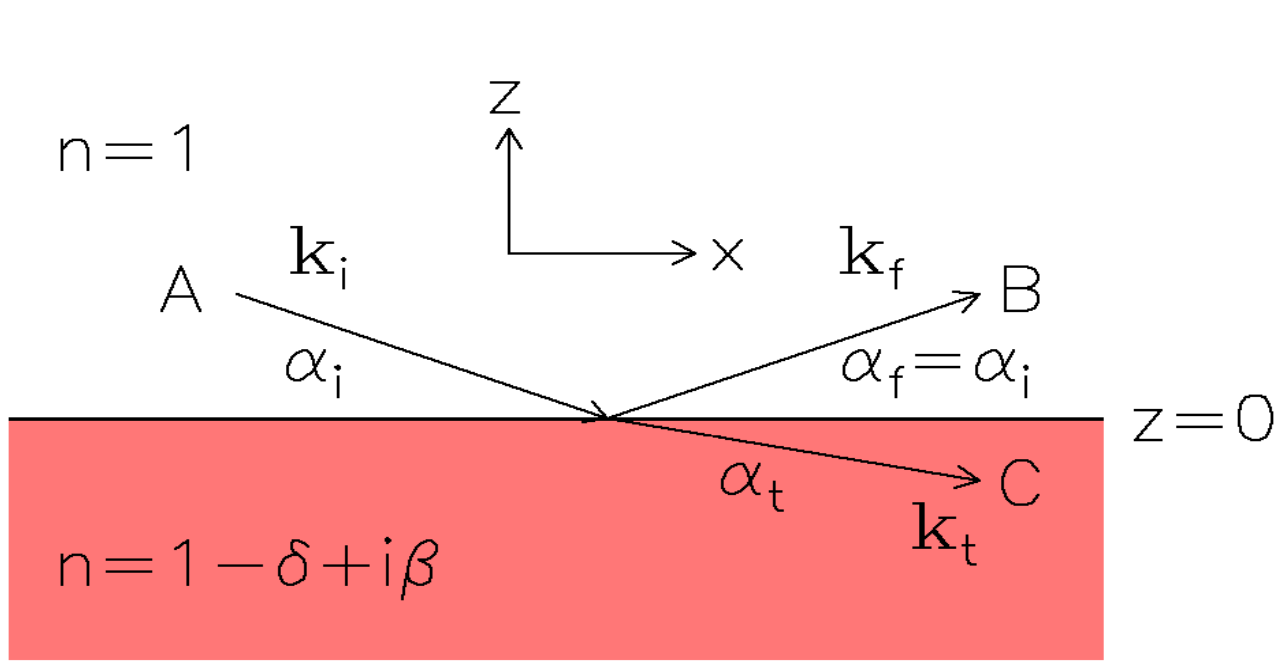
\includegraphics[width=\textwidth]{bilder/einschicht.png}
  \caption{Übergang einer elektromagnetischen Welle vom Vakuum in ein
            anderes Medium und dabei auftretetende Reflexion und Transmission.\cite{sample}}
  \label{fig:einschicht}
\end{figure}
\FloatBarrier

In Abbildung \ref{fig:einschicht} wird für das Ursprungsmedium das Vakuum gewählt,
sodass gilt $n_{1} = 1$. Für den Brechungsindex $n_{2}$ des anderen Mediums,
wird eine komplexe Zahl
\begin{align}
  n_{2} = \alpha + i \beta& &\text{mit } \alpha, \beta \in \mathbb{N}
  \label{eqn:komplexerindex}
\end{align}
gewählt. Der Realteil $\alpha$ beinhaltet die Informationen bezüglich der eigentlichen
Brechung und der Imaginarteil $\beta$ die Dämpfung der Welle im Medium. Für Röntgenstrahlung
gilt typischerweise $\alpha < 1$. Dies liegt daran, dass der reele
Brechungsindex das Verhältnis von Lichtgeschwindigkeit im Medium zu der im Vakuum
misst und für Röntgenstrahlung die Phasengeschwindigkeit im Medium
schneller sein kann als die Vakuumlichtgeschwindigkeit $c_{0}$.
Da der Realteil von $n$ den Wert $1$ nur um sehr kleine Werte
$\delta \sim 10^{-6}$ unterschreitet, wird die Formulierung
$\alpha = 1 - \delta$ gewählt,
sodass aus Gleichung \eqref{eqn:komplexerindex},
\begin{align}
  n_{2} = 1 - \delta + i \beta
  \label{eqn:komplexerindexdelta}
\end{align}
wird.

% kritischer Winkel
Anhand des Brechungsgesetzes \eqref{eqn:snellius} wird klar , dass ein Winkel
$\alpha_\text{{crit.}}$ existiert, bei dem die Welle nicht in das
zweite Medium eintritt, also total refelektiert wird.

% fresnel -> transmissions/reflektions amplituden -> Fresnelreflektivitaet



% dag
\subsection{Brechung von Röntgenstrahlung in Mehrschichtsystemen}
\label{subsec:mehrschicht}

% Reflektivitaet + Kiessig-Ringe


% rekursionszeug + Gesamtreflektivitaet


\subsection{Rauigkeit}
\label{subsec:rauigkeit}





\cite{sample}
